\section{Versuchsaufbau}
Der verwendete Versuchsaufbau ist in Abbildung $\ref{fig:Aufbau}$ dargestellt. Die von der
Strahlungsquelle $\ce{^{241} Am}$ ausgehenden $\alpha$-Teilchen werden durch zwei $\SI{2}{\mm}$
Schlitzblenden fokussiert, bevor sie eine dünne Goldfolie erreichen, an der sie gestreut werden.
Die gestreuten Teilchen werden mit einem Surface-Barrier Detektor in Abhängigkeit des Streuwinkels
detektiert. Da $\alpha$-Teilchen in Luft nur eine Reichweite von ca. $\SI{1,5}{\cm}$ haben, wird der gesamte
Versuch im Vakuum durchgeführt.
\begin{figure}
  \centering
  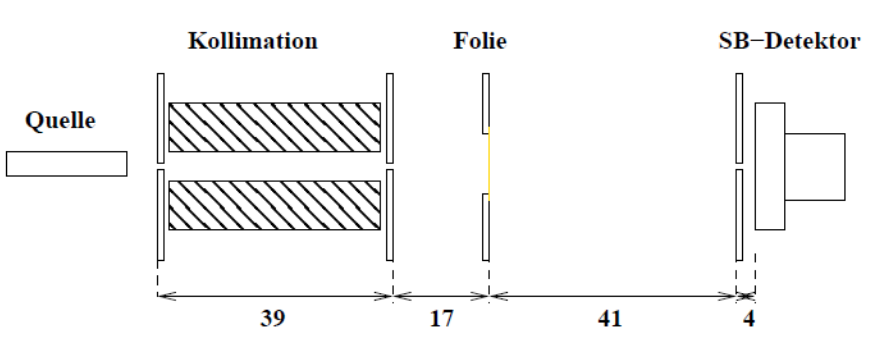
\includegraphics[width=11cm]{Aufbau.png}
  \caption{Darstellung der verwendeten Messapparatur.}
  \label{fig:Aufbau}
  \cite{skript}
\end{figure}

\section{Durchführung}
Zunächst wird wird die Vakuumapparatur evakuiert und die Sperrspannung des Surface-Barrier Detektors auf
$U_{det}=\SI{12}{\V}$ eingestellt. Um die Anstiegsteiten der Pulse zu vermessen und die Energieverlustmessung
durchzuführen wird zunächst ein Oszilloskop angeschlossen. Die Anstiegszeiten können direkt abgelesen werden.
Für die Energieverlustmessung wird die Pulshöhe der Detektorpulse in Abhängigkeit des Drucks vermessen. Um
daraus später die Foliendicke bestimmen zu können wird diese Messung einmal mit eine 2\:$\symup{\mu}$m dicken
Au-Folie und einmal ohne Folie durchgeführt.

Um im Folgenden den differentielle Streuquerschnitt der 2\:$\symup{\mu}$m Au-Folie zu bestimmen wird nun ein Zähler
angeschlossen. Der Detektor wird in Schritten von $\SI{1}{\degree}$ von $\SI{-17}{\degree}$ bis $\SI{17}{\degree}$
verschoben, während der Zähler die Zählrate $I$ jeweils in einem Zeitintervall von $\SI{360}{\s}$ misst.

Um anschließend den Einfluss der Mehrfachstreuung zu untersuchen wird nun ein fester Winkel von ???$\SI{2}{\degree}$
gewählt, an dem die Zählrate einer 4\:$\symup{\mu}$m dicken Au-Folie für $\SI{360}{\s}$ gemessen wird.

Abschließend wird die Z-Abhängigkeit an den Materialien Bismut und Aluminium untersucht. Dazu wird die Zählrate
bei einem festen Winkel von $\SI{7}{\degree}$ ebenfalls für $\SI{360}{\s}$ vermessen.


\section{Vorbereitung}
\textbf{Energieverlust und Reichweite von $\alpha$-Strahlung in Luft}\\
Der Energieverlust der $\alpha$-Strahlung in Luft kann mithilfe der Bethe-Bloch Formel \ref{eqn:BetheBloch} berechnet
werden. Unter Berücksichtigung der Luftzusammensetzung (78\% Stickstoff und 20\% Sauerstoff) ergibt sich für
Luft eine Ordnungszahl von $Z_{\text{Luft}}=7,06$, eine Massenzahl von $A_{\text{Luft}}=14,12$ und eine
mittlere Ionisationsenergie von $I_{\text{Luft}}=\SI{14,05}{\eV}$.
Die Dichte von Luft beträgt $\rho_{\text{Luft}}=\SI{1,204}{\kg\per\m^3}$. Daraus kann nach der Formel

\begin{equation}
  N=\frac{\rho}{m_{\text{Atom}}}
  \label{eqn:Anzahl}
\end{equation}
mit $m_{\text{Atom}}=A\cdot u$ die Teilchenzahl berechnet werden, wobei $u$ die
atomare Masseneinheit bezeichnet. Somit ergibt sich für Luft eine Teilchenzahl von

\begin{equation}
  N=\SI{5,54e25}{\per\m^3}.
\end{equation}
Insgesamt lässt sich daraus ein Energieverlust von
\begin{equation}
  -\frac{dE}{dx}=\SI{-138,19}{\kilo\eV\per\mm}
\end{equation}
berechnen.

Um daraus die Reichweite in Luft bestimmen zu können wird die Formel
\begin{equation}
  0=E_{\alpha}-R\cdot\frac{dE}{dx}
\end{equation}
nach
\begin{equation}
  R=\frac{E_{\alpha}}{\frac{dE}{dx}}
\end{equation}
umgestellt.

Für eine Anfangsenergie der $\alpha$-Teilchen ergibt sich somit in Luft eine
Reichweite von $R=\SI{3,97}{\cm}$.

Im Folgenden soll die Abhängigkeit der Energieverlustmessung vom Druck bestimmt werden, dazu
wird die Gleichung
\begin{equation}
N=\frac{pV}{RT}
\end{equation}
verwendet, welche aus der idealen Gasgleichung $pV=NRT$ folgt. Das Volumen $V$ kann
dabei über $V=\sfrac{M}{\rho}$ bestimmt werden. Durch einsetzen in die Formel \ref{eqn:BetheBloch}
erhält man folgenden Ausdruck:

\begin{equation}
  -\frac{dE}{dx}=-\frac{4\pi e^4 z^2 p MZ}{m_0 v^2 R\rho T (4\pi\epsilon_0)^2}\cdot\Big(\frac{2m_0v^2}{I}).
  \label{eqn:BetheBlochDruck}
\end{equation}

Anhand dieser Formel wird deutlich, dass der Energieverlust direkt proportional zum
Druck ist. Um zu bestimmen, ab welchem Druck der Energieverlust bemerkbar wird, wird
Formel \ref{eqn:BetheBlochDruck} nach $p$ umgeformt. Mit den Annahmen, dass der Energieverlust
ab $\SI{1}{\kilo\eV}$ pro $\SI{100}{\mm}$ relevant wird erhält man durch einsetzen eine
Druckdifferenz von
\begin{equation}
  \Delta p=\SI{12,04}{\Pa}.
\end{equation}
